\usetikzlibrary{positioning}
\usetikzlibrary{arrows.meta}
\usetikzlibrary{bending}
\definecolor{red}{HTML}{8A3F3A}
\definecolor{yellow}{HTML}{E0BB3C}
\definecolor{blue}{HTML}{4569E0}
\definecolor{green}{HTML}{17E561}
\definecolor{other}{HTML}{6A939E}

% DTU Colors
\definecolor{dtu-corporate-red}{HTML}{990000}
\definecolor{dtu-white}{HTML}{ffffff}
\definecolor{dtu-black}{HTML}{000000}
\definecolor{dtu-blue}{HTML}{2F3EEA}
\definecolor{dtu-bright-green}{HTML}{1FD082}
\definecolor{dtu-navy-blue}{HTML}{030F4F}
\definecolor{dtu-yellow}{HTML}{F6D04D}
\definecolor{dtu-orange}{HTML}{FC7634}
\definecolor{dtu-pink}{HTML}{F7BBB1}
\definecolor{dtu-grey}{HTML}{DADADA}
\definecolor{dtu-red}{HTML}{E83F48}
\definecolor{dtu-green}{HTML}{008835}
\definecolor{dtu-purple}{HTML}{79238E}


\newlength{\basisb}
\setlength{\basisb}{0.4cm}

\centering
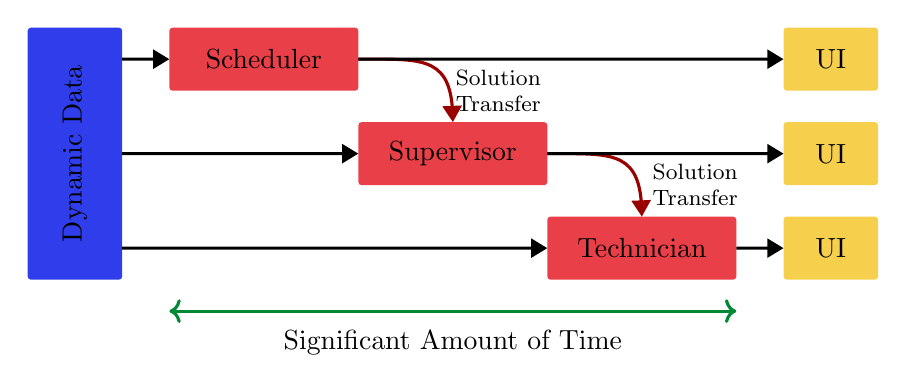
\begin{tikzpicture}[line width=0.0\basisb]
    \draw (2.0\basisb,4.0\basisb) 
		node[rotate=90, minimum height=3\basisb,fill=dtu-blue,minimum width=8\basisb,rounded corners=0.1\basisb] 
			(Dynamic Data) {Dynamic Data};

    \draw (8.0\basisb,7.0\basisb) 
		node[minimum height=2\basisb,fill=dtu-red,minimum width=6\basisb,rounded corners=0.1\basisb] 
			(Scheduler) {Scheduler};
    \draw (14.0\basisb,4.0\basisb) 
		node[minimum height=2\basisb,fill=dtu-red,minimum width=6\basisb,rounded corners=0.1\basisb] 
			(Supervisor) {Supervisor};
    \draw (20.0\basisb,1.0\basisb) 
		node[minimum height=2\basisb,fill=dtu-red,minimum width=6\basisb,rounded corners=0.1\basisb] 
			(Technician) {Technician};

    \draw (26.0\basisb,7.0\basisb) 
		node[minimum height=2\basisb,fill=dtu-yellow,minimum width=3\basisb,rounded corners=0.1\basisb] 
			(UserInterface1) {UI};
    \draw (26.0\basisb,4.0\basisb) 
		node[minimum height=2\basisb,fill=dtu-yellow,minimum width=3\basisb,rounded corners=0.1\basisb] 
			(UserInterface2) {UI};
    \draw (26.0\basisb,1.0\basisb) 
		node[minimum height=2\basisb,fill=dtu-yellow,minimum width=3\basisb,rounded corners=0.1\basisb] 
			(UserInterface3) {UI};

	\draw[<->, line width=0.1\basisb,color=dtu-green] (5.0\basisb, -1\basisb) -- (23.0\basisb, -1\basisb);
	\draw (14.0\basisb, -2.0\basisb) node {Significant Amount of Time};

	\draw[->,>=Triangle, thick, line width=0.1\basisb, color=dtu-corporate-red] (Scheduler) to[out=0, in=90,looseness=1.5]  (Supervisor);
	\draw[->,>=Triangle, thick, line width=0.1\basisb, color=dtu-corporate-red] (Supervisor) to[out=0, in=90,looseness=1.5] (Technician);
	\draw[->,>=Triangle, thick, line width=0.1\basisb] (Dynamic Data.south) ++(0\basisb,3.0\basisb) to[out=0, in=180,looseness=1.0] (Scheduler);
	\draw[->,>=Triangle, thick, line width=0.1\basisb] (Dynamic Data.south) to[out=0, in=180,looseness=1.0] (Supervisor);
	\draw[->,>=Triangle, thick, line width=0.1\basisb] (Dynamic Data.south) ++(0\basisb,-3.0\basisb) to[out=0, in=180,looseness=1.0] (Technician.west);
	\draw[<-,>=Triangle, thick, line width=0.1\basisb] (UserInterface1) to[out=180, in=0,looseness=1.0] (Scheduler);
	\draw[<-,>=Triangle, thick, line width=0.1\basisb] (UserInterface2) to[out=180, in=0,looseness=1.0] (Supervisor);
	\draw[<-,>=Triangle, thick, line width=0.1\basisb] (UserInterface3) to[out=180, in=0,looseness=1.0] (Technician);
	% \draw[<->, thick, line width=0.1\basisb] (Scheduler) -- (UserInterface);
	\begin{scope}[shift={(7,0)}] % Adjust shift to position the legend
    % Legend box
    % Legend lines and text
	    \draw[thick, line width=0.1\basisb] (-1.5,2.4) node[right, font=\footnotesize, align=center] {Solution\\Transfer};
	    \draw[thick, line width=0.1\basisb] (1.0,1.2) node[right, font=\footnotesize, align=center] {Solution\\Transfer};
	\end{scope}
\end{tikzpicture}
